% ★★★ 难题
\newcommand{\qConicHardNewGaokaoStem}{
已知椭圆 $C: \frac{x^2}{a^2} + \frac{y^2}{b^2} = 1$ ($a > b > 0$) 的离心率为 $\frac{\sqrt{2}}{2}$，且过点 $A(2, 1)$．
(1) 求 $C$ 的方程；
(2) 点 $M, N$ 在 $C$ 上，且 $AM \perp AN$，$AD \perp MN$，$D$ 为垂足．证明：存在定点 $Q$，使得 $|DQ|$ 为定值．
}
\newcommand{\qConicHardNewGaokaoFigure}{
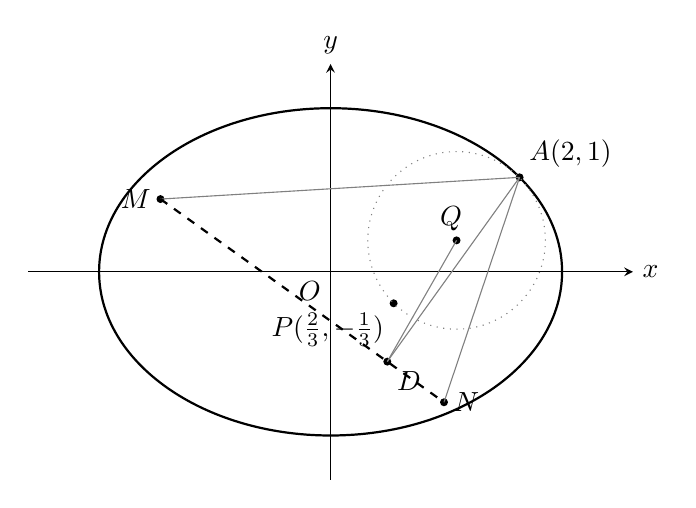
\begin{tikzpicture}[scale=1.2, >=stealth]
  % Axes
  \draw[->] (-3.2,0) -- (3.2,0) node[right] {$x$};
  \draw[->] (0,-2.2) -- (0,2.2) node[above] {$y$};
  \node[below left] at (0,0) {$O$};
  
  % Ellipse: x^2/6 + y^2/3 = 1 => a=2.45, b=1.732
  \draw[thick] (0,0) ellipse (2.45 and 1.732);
  
  % Points A(2, 1)
  \coordinate (A) at (2.0, 1.0);
  \fill (A) circle (1.2pt) node[above right] {$A(2, 1)$};
  
  % Fixed Point P(2/3, -1/3)
  \coordinate (P) at (0.667, -0.333);
  \fill (P) circle (1.2pt) node[below left] {$P(\frac{2}{3}, -\frac{1}{3})$};
  
  % Fixed Point Q(4/3, 1/3) which is midpoint of AP
  \coordinate (Q) at (1.333, 0.333);
  \fill (Q) circle (1.2pt) node[above, xshift=-2pt] {$Q$};
  
  % Let's draw M and N on the ellipse such that AM \perp AN
  % Let's pick M and N. For example, M(-2.0, 0.577) approx on ellipse
  % Since AM \perp AN, let's show MN line and foot D
  \coordinate (M) at (-1.8, 0.77);
  \coordinate (N) at (1.2, -1.38);
  \fill (M) circle (1.2pt) node[left] {$M$};
  \fill (N) circle (1.2pt) node[right] {$N$};
  
  % Draw lines AM and AN
  \draw[thin, gray] (A) -- (M);
  \draw[thin, gray] (A) -- (N);
  
  % Draw hypotenuse MN
  \draw[thick, dashed] (M) -- (N);
  
  % Draw foot D of perpendicular from A onto MN
  % Line MN: y - 0.77 = (-1.38-0.77)/(1.2-(-1.8)) * (x - (-1.8)) => y - 0.77 = -0.717*(x+1.8) => y = -0.717x - 0.52
  % Perpendicular from A(2, 1): y - 1 = 1.395*(x - 2) => y = 1.395x - 1.79
  % Intersection D: -0.717x - 0.52 = 1.395x - 1.79 => 2.112x = 1.27 => x_D = 0.60, y_D = -0.95
  \coordinate (D) at (0.60, -0.95);
  \fill (D) circle (1.2pt) node[below right] {$D$};
  \draw[thin, gray] (A) -- (D);
  
  % Circle with diameter AP, centered at Q, radius = 0.94
  \draw[dotted, gray] (Q) circle (0.94);
  \draw[thin, gray] (Q) -- (D);
\end{tikzpicture}
}
\newcommand{\qConicHardNewGaokaoAnswer}{
(1) 椭圆 $C$ 的方程为 $\frac{x^2}{6} + \frac{y^2}{3} = 1$．\\
(2) 证明见解析，存在定点 $Q(\frac{4}{3}, \frac{1}{3})$，使得 $|DQ| = \frac{2\sqrt{2}}{3}$ 为定值．
}
\newcommand{\qConicHardNewGaokaoSolution}{
\begin{proof*}
(1) 设椭圆 $C$ 的半焦距为 $c$．由离心率 $e = \frac{c}{a} = \frac{\sqrt{2}}{2}$，得 $a^2 = 2c^2$．\\
因为 $a^2 = b^2 + c^2$，所以 $2c^2 = b^2 + c^2 \implies b^2 = c^2$．故 $a^2 = 2b^2$．\\
所以椭圆 $C$ 的方程为 $\frac{x^2}{2b^2} + \frac{y^2}{b^2} = 1$．\\
将点 $A(2, 1)$ 代入方程得：
\[
\frac{4}{2b^2} + \frac{1}{b^2} = 1 \implies \frac{3}{b^2} = 1 \implies b^2 = 3
\]
所以 $a^2 = 2b^2 = 6$．\\
故椭圆 $C$ 的方程为 $\frac{x^2}{6} + \frac{y^2}{3} = 1$．\\

(2) 设直线 $MN$ 的方程为一般式 $l: Ax + By + C = 0$．\\
由点 $A(2, 1)$ 不在直线 $MN$ 上，可知 $2A + B + C \neq 0$．\\
椭圆 $C$ 的标准方程参数为 $a^2 = 6$（$x^2$ 分母），$b^2 = 3$（$y^2$ 分母）．\\
此时统一分母为 $D = A^2a^2 + B^2b^2 = 6A^2 + 3B^2$．\\
设 $M(x_1, y_1), N(x_2, y_2)$，联立直线与椭圆方程，直接代入硬解定理公式可写出交点坐标的韦达结构：
\[
x_1 + x_2 = -\frac{2ACa^2}{D} = -\frac{12AC}{D},\qquad x_1x_2 = \frac{a^2(C^2 - B^2b^2)}{D} = \frac{6(C^2 - 3B^2)}{D}
\]
\[
y_1 + y_2 = -\frac{2BCb^2}{D} = -\frac{6BC}{D},\qquad y_1y_2 = \frac{b^2(C^2 - A^2a^2)}{D} = \frac{3(C^2 - 6A^2)}{D}
\]
通过硬解公式，我们将极其复杂的消元和展开工作直接转化为上述四个对称量，简化了繁重的计算．\\
根据垂直条件 $AM \perp AN$，在向量上表示为 $\vec{AM} \cdot \vec{AN} = 0$，即：
\[
(x_1 - 2)(x_2 - 2) + (y_1 - 1)(y_2 - 1) = 0 \implies x_1x_2 + y_1y_2 - 2(x_1 + x_2) - (y_1 + y_2) + 5 = 0
\]
将硬解定理公式代入上式中：
\[
\frac{6(C^2 - 3B^2)}{D} + \frac{3(C^2 - 6A^2)}{D} - 2\left(-\frac{12AC}{D}\right) - \left(-\frac{6BC}{D}\right) + 5 = 0
\]
两边同乘以分母 $D = 6A^2 + 3B^2$：
\[
6(C^2 - 3B^2) + 3(C^2 - 6A^2) + 24AC + 6BC + 5(6A^2 + 3B^2) = 0
\]
展开并合并同类项：
\[
6C^2 - 18B^2 + 3C^2 - 18A^2 + 24AC + 6BC + 30A^2 + 15B^2 = 0
\]
\[
12A^2 - 3B^2 + 9C^2 + 24AC + 6BC = 0
\]
两边除以 $3$，化简得到关于 $A, B, C$ 的二次齐次关系式：
\[
4A^2 - B^2 + 3C^2 + 8AC + 2BC = 0
\]
我们将此式视为关于 $C$ 的一元二次方程进行因式分解：
\[
3C^2 + 2(4A + B)C + (4A^2 - B^2) = 0
\]
计算其判别式：
\[
\Delta_C = 4(4A + B)^2 - 12(4A^2 - B^2) = 4(16A^2 + 8AB + B^2) - 48A^2 + 12B^2 = 16A^2 + 32AB + 16B^2 = 16(A+B)^2
\]
判别式为完全平方式，解得 $C$ 关于 $A, B$ 的线性关系：
\[
C = \frac{-2(4A+B) \pm 4(A+B)}{6} = \frac{-(4A+B) \pm 2(A+B)}{3}
\]
解得：
\[
C = -2A - B \quad \text{或} \quad C = \frac{-2A+B}{3}
\]
若 $C = -2A - B$，则 $2A + B + C = 0$，此时直线 $Ax+By+C=0$ 恒过点 $A(2, 1)$，与点 $M, N$ 为椭圆上不同于 $A$ 的两点矛盾，舍去．\\
因此必有 $3C + 2A - B = 0$，即 $\frac{2}{3}A - \frac{1}{3}B + C = 0$．\\
这说明直线 $MN$ 恒过定点 $P(\frac{2}{3}, -\frac{1}{3})$．\\
因为 $AD \perp MN$，所以 $\angle ADP = 90^\circ$，即垂足 $D$ 在以线段 $AP$ 为直径的圆上．\\
定点 $A(2, 1)$ 与定点 $P(\frac{2}{3}, -\frac{1}{3})$ 确定的线段 $AP$ 中点为圆心 $Q$，其坐标为：
\[
Q\left(\frac{2 + \frac{2}{3}}{2}, \frac{1 - \frac{1}{3}}{2}\right) \implies Q\left(\frac{4}{3}, \frac{1}{3}\right)
\]
直径长度为：
\[
|AP| = \sqrt{\left(2 - \frac{2}{3}\right)^2 + \left(1 - \left(-\frac{1}{3}\right)\right)^2} = \sqrt{\frac{16}{9} + \frac{16}{9}} = \frac{4\sqrt{2}}{3}
\]
所以圆的半径为 $R = \frac{1}{2}|AP| = \frac{2\sqrt{2}}{3}$．\\
根据圆的几何性质，圆上任意点 $D$ 到圆心 $Q$ 的距离恒等于半径 $R$，即存在定点 $Q\left(\frac{4}{3}, \frac{1}{3}\right)$，使得 $|DQ| = \frac{2\sqrt{2}}{3}$ 为定值．
\end{proof*}
}
\newcommand{\qConicHardNewGaokaoDiagnosis}{
\errortag{硬解一般式直接化简} 本题如果采用常规纵截式 $y=kx+m$ 联立，由于 $A(2,1)$ 坐标非零，式子中会包含极其杂乱的交叉项、一次项和常数项，代数通分计算量呈指数级增长，极易算错。若采用硬解一般式直线 $Ax+By+C=0$，直接代入四个基本韦达对称量，能够瞬间将问题转化为 $A, B, C$ 的二次齐次式。关键在于利用判别式 $\Delta_C = 16(A+B)^2$ 是完全平方式，将二次式分解为两个一次因式，从而锁定直线过定点。这一代数推导过程简洁严密，完美体现了硬解定理统摄一般式直线的计算优势．\\
\errortag{几何直角转化为圆} 第 (2) 问中求 $|DQ|$ 的定值，如果直接写出 $D$ 的坐标并用两点距离公式硬算，会由于 $D$ 在动直线上而导致极度复杂的根式计算。通过发现 $\angle ADP = 90^\circ$ 并转化为“直角所对的弦为圆直径”，将 $D$ 的轨迹锁定为定圆，从而使 $|DQ|$ 直接转化为圆的半径，无需进行任何复杂的代数运算。
}

